\cleardoublepage
\newrefsection
\chapter{文献综述}

\section{背景介绍}

随着晶体管的组件尺寸越来越接近物理极限,现代计算机的性能提升放缓,因此多核CPU被提出用于提出计算机整体性能。并发编程本来是用于在单个CPU上同时运行多个任务的技术,合理的并发编程有助于提升CPU的利用效率。但是并发程序的引入也导致了新的安全问题,即在并发程序的运行过程中不同线程的执行序列不确定,进而可能导致数据争用等问题,但是由于并发程序导致的安全问题需要特定的执行序列才能显现出来,这使得发现并发程序漏洞十分困难。而fuzzing技术可以有效地探索并发访问漏洞,因此这方面的技术十分重要,目前也已经有大量的工作致力于发现并发访问漏洞。

\subsection{模糊测试}

模糊测试是一种用来测试程序或者计算机系统是否存在问题的技术,其核心思想是对自动生成一段随机数据输入到程序之中,并观察程序是否会出现异常(例如崩溃),并基于此发现可能的程序错误。

模糊测试主要分为以下几个部分:
\begin{enumerate}
\item 输入生成器:用于生成程序的输入。例如通过随机生成器创建大量的输入数据,包括各种数据类型和格式,以达到涵盖系统可能遇到的各种情况的目的。
\item 执行器:利用上一步的输入进行实际程序的执行。在这个过程中模拟系统的输入,可能涉及到用户输入、网络通信、文件读取等。
\item 反馈监控:在程序运行时或程序运行结束之后检测是否有异常发生。通过记录系统对输入的反应,包括崩溃、异常行为、错误信息、资源占用情况等信息,进而分析系统是否发生了异常的行为。同时这些信息也可以为输入生成器提供反馈,生成新的输入。
\end{enumerate}

如\autoref{fig:fig1}所示

\begin{figure}[ht]
    \centering
    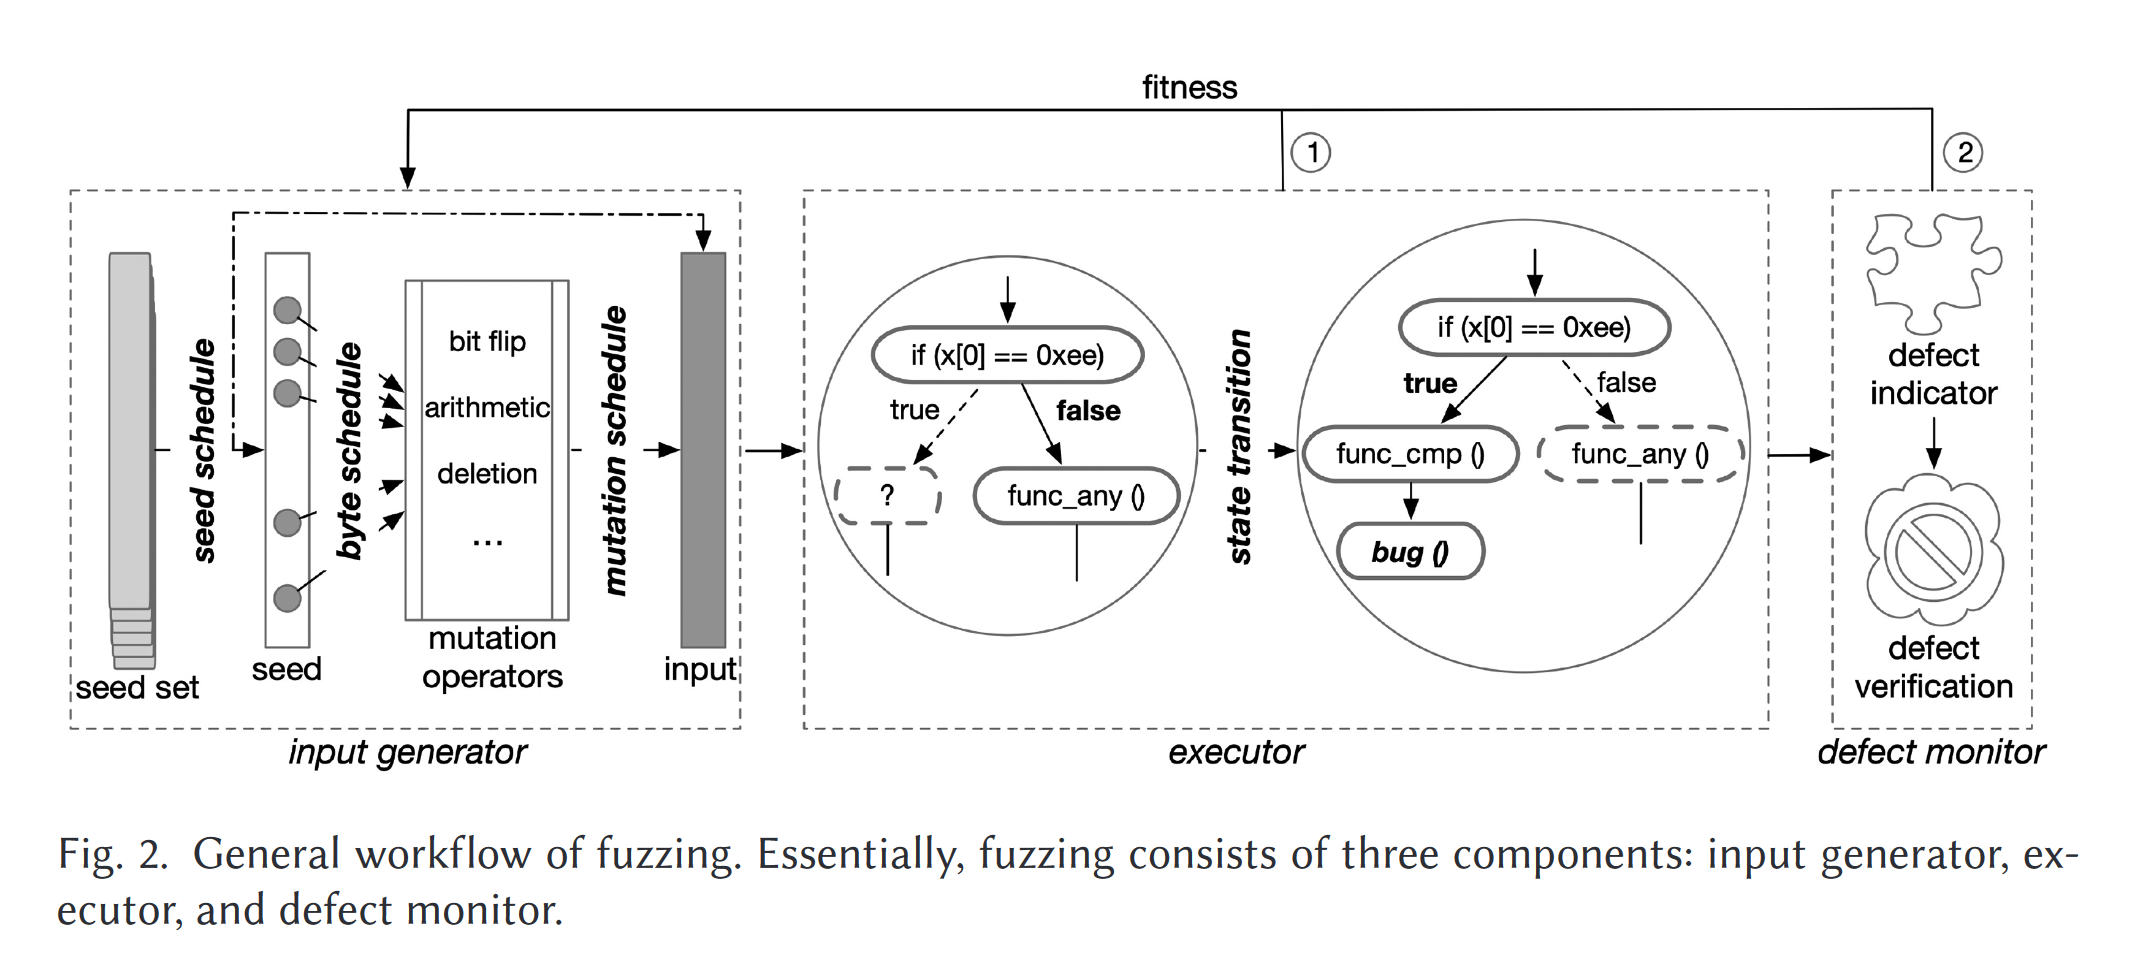
\includegraphics[width=0.8\linewidth]{fig1}
    \caption{\label{fig:fig1}模糊测试的系统组成}
\end{figure}

在模糊测试系统运行时,首先生成示例输入,然后利用输入运行程序,并在程序运行过程中进行监视,如果过程中发现异常,则将这一个输入记录下来。并利用获得的信息生成下一轮测试所需的输入,再次进行测试。

在实际应用中,模糊测试通常结合了生成测试和变异测试的思想。它可以应用于各种软件系统,包括应用程序、操作系统、驱动程序、网络协议等,以帮助发现并修复潜在的安全漏洞和软件缺陷。总的来说,模糊测试是一种强大的测试方法,可以帮助提高软件系统的健壮性和安全性,尤其是对于大规模、复杂的软件系统来说,模糊测试具有重要的意义。

\subsubsection{基于输入生成方法的分类}

从输入生成方法上可以将模糊测试分为两类,一类是生成测试,另一类是变异测试。

生成测试通过对程序输入进行建模,基于这个建模来生成新的测试数据。例如,可以使用随机生成的输入,或者基于输入的特定规则来生成输入。这种方法则是基于已有的输入,通过对其进行修改或变异来生成新的输入。这些变异可能涉及对输入的一些微小改变,比如改变数据的顺序、插入、删除或替换数据等。这两种方法可以单独或结合使用,以实现对系统的全面测试覆盖。生成测试通常用于探索输入空间的广度,而变异测试则侧重于探索输入空间的深度,从而共同促进系统的健壮性和可靠性。

\subsubsection{基于获取信息量的分类}

从程序运行时获取的信息量的角度可以将模糊测试分为三类,分别是黑盒模糊测试,白盒模糊测试,灰盒模糊测试。

黑盒模糊测试对于程序运行时的内部状态没有任何的信息,只有输入和输出的状态信息。这种测试在速度上最快,因为不需要去收集程序执行时的信息,但是代价就是无法根据程序运行时的信息生成更加有效的测试用例。

白盒模糊测试拥有程序运行时完整的内部状态信息,并利用这些信息对程序的状态空间进行完全的探索,通常会结合动态符号执行来进行分析。但是这样会带来很大的测试开销。

灰盒模糊测试获取介于白盒和黑盒测试之间的信息量,例如边缘覆盖率,函数覆盖率等等,利用这些信息来指导输入的生成。这种方式在性能和准确度上进行了平衡。

\subsection{利用模糊测试挖掘漏洞}

\subsubsection{模糊测试应用的领域}

\begin{enumerate}
\item 信息安全。模糊测试被用于发现系统中的安全漏洞,如缓冲区溢出、代码注入等。也被用于对防火墙、入侵检测系统等安全产品进行测试,以评估其对各种攻击的抵御能力。
\item 网络协议。模糊测试用于测试网络协议的安全性,以发现可能的漏洞和攻击面。对通信软件、网络服务器等进行模糊测试,以确保其在各种情况下都能正常运行。
\item 物联网设备。对智能家居设备和系统进行模糊测试,以发现可能的安全隐患。测试物联网设备和嵌入式系统,以确保其稳定性和安全性。
\item 操作系统。模糊测试用于测试操作系统内核,以发现可能的漏洞和异常行为。对操作系统的各个部分(如驱动、文件系统等)进行模糊测试,保证其稳定性和兼容性。
\item Web应用程序。对Web浏览器进行模糊测试,以确保其对恶意网站和恶意脚本的抵御能力。同时也用于测试Web程序的安全性,检测可能的漏洞和攻击面。
\end{enumerate}

\subsubsection{利用模糊测试挖掘并发访问程序漏洞}

对于并发访问程序来说,通常的模糊测试并不能充分探索并发访问下的数据争用,因为数据争用需要特定的线程执行顺序才能被触发,但是通常情况下的模糊测试仅仅只是生成不同的输入,而并没有考虑到线程的交错顺序。因此如果要对并发程序进行模糊测试,还需要探索到线程的交错空间。这里就涉及到几个问题:

\begin{enumerate}
\item 精准控制程序在特定位置进行线程切换。在通常执行情况下,线程的切换由操作系统控制,操作系统根据动态的信息选择是否进行线程切换,以及切换到哪一个线程。因此如何控制不同的线程在特定位置暂停运行并切换到下一个线程运行是探索线程交错空间必须要解决的问题。
\item 探索空间过大,不可能在合理时间内对所有情况进行探索。对于多个线程来说,考虑到线程的指令数量以及线程的数量,交错空间包含的数量随线程的数量增加呈阶乘趋势上升,因此要在合理时间内对所有的情况进行探索是不可能的,因此需要通过其他方式对探索进行指导,使其能够更加有效地在空间内探索。
\item 检测是否产生了错误。在程序运行过程中产生错误的表现有很多种,最明显的一种就是系统无法正常运行。但是还有很多情况是系统虽然出现了问题,但是没有以一种明显的方式表现出来(如内存泄漏等),这种情况下即使出现了问题也不能被我们发现。因此需要能够在模糊测试的过程中检测是否产生了具体的问题。
\end{enumerate}

由于以上的问题,在利用模糊测试挖掘并发访问程序漏洞的时候,不能简单地将通用的模糊测试应用到并发程序上,这方面目前已经有一些研究,但是对于并发访问程序的漏洞仍然不能做到很好的挖掘,仍然需要更多的探索。

\section{国内外研究现状}

\subsection{研究方向及进展}

\subsubsection{交错空间优化输入生成}

2019年,Jeong\cite{jeong2019razzer}等人开发了Razzer,通过静态分析(point-to analysis)识别,得到所有可能产生冲突的指令对,即可能访问同一个地址的属于不同线程的两条指令,并得到所有可能产生冲突的指令对集合。然后进行单线程模糊测试以得到可以使程序执行到特定访存指令的输入。然后进行多线程测试,利用单线程测试得到的输入以及断点插入,使得程序按照规划好的顺序交错执行,然后观察是否会让程序发生异常或者其他错误。相比于Syzkaller,这一方法可以用更少的变异、执行次数找到更多的有效bug。但是Razzer的执行速度相比于Syzkaller更慢,并且利用point-to-analysis可能无法找到所有的冲突指令对.

\subsubsection{改进交错空间反馈指标}

2020年,Hongxu Chen\cite{chen2020muzz}等人提出了MUZZ,这篇文章首先通过静态分析得到可能会产生冲突的scope,然后对这些scope进行插桩。然后进行fuzzing的过程,利用前面插桩的代码,得到代码覆盖率,线程上下文,交错顺序三个信息,并根据这些信息进行种子的选择,排序,变异,生成新的测试用例。最后利用T-Sanitize检测漏洞。相比于之前的工作,MUZZ能够产生出更多和多进程相关的种子,也就是说能够测试更多多线程的用例。同时相比于AFL等工具能够检测出更多的数据争用缺陷。

2020年,Meng Xu\cite{xu2020krace}等人提出了KRACE,通过引入一个新的覆盖跟踪指标,别名覆盖率,来捕获并发维度的探索进度。通过这个新的维度,结合一种用于生成、变异、合并多线程系统调用序列的进化算法,引导fuzzer对线程并发空间进行更有效的探索。相对于Syzkaller,KRACE可以发现更多的branch path。但是也会引入更大的开销。

2022年,Zu-Ming Jiang\cite{jiang2022context}等人通过引入并发调用对这个新的并发覆盖指标,确保上下文敏感性,并提出了一种邻接导向突变,生成新的可能的线程交错。这篇文章提出了CONZZER框架,并在8个用户级程序和4个内核级文件系统上进行了测试,并发现了95个数据竞争,其中75个是有害的。

2023年,Jeong等人提出SEGFUZZ\cite{jeong2023segfuzz},将对整个线程的交错空间进行分解,对一小段代码进行探索,然后再将多个小段代码合并再进行探索,并提出交织段覆盖率的概念,再提高发现并发错误的准确性的同时,避免了冗余测试。这很大程度上降低了并发空间探索的复杂度。SEGFUZZ在linux内核中发现了21个新的并发错误,并且这些错误都表现出有害行为。并且相对于Snowboard和KRACE这些之前的工作能够更快地发现并发错误(平均快4.1倍)

2023年,Ming Yuan等人开发了DDRACE\cite{yuan2023ddrace},提出了新的距离度量反馈,RPIP(Race Pair Interaction Profile)反馈,约束反馈,来指导生成新的输入,并利用一种交错优先级方案来选择更有可能产生并发访问缺陷的输入。相对于Syzkaller,RAZZER,KRACE这些工具,DDRACE可以发现更多的并发访问缺陷,并且可以在更短时间内发现。

\subsection{存在问题}

\begin{enumerate}
\item 对于线程交错空间的探索并不充分且有效,由于线程交错空间过大,因此只能尽可能在空间中进行有效的探索,当前的技术都不能很好地尽可能进行有效的探索。
\item 尽管目前的研究提出了很多种新的反馈指标来指导Fuzzer生成能够进行更深入空间探索的输入,但是这些反馈指标在性能和有效性上不能做到很好的平衡,往往比较好的效果会引入很大的开销,包括内存和处理器资源,尤其是在模拟大规模并发访问的情况下。这可能会对测试环境和目标系统造成一定压力。
\item 由于并发访问程序中的问题通常依赖于特定的并发条件和时序,因此有时很难通过模糊测试来准确重现问题,特别是对于一些偶发的并发漏洞。
\item 并发模糊测试产生的大量测试数据和结果需要进行有效的分析和处理。发现并发漏洞并确定其严重性需要耗费大量时间和精力。
\end{enumerate}

\section{研究展望}

\begin{enumerate}
\item 随着人工智能和机器学习的发展,可以通过建立模型的方式,这些模型可以根据以往的测试结果和模式,自动调节测试策略,从而提升测试的效率和效果,进而帮助发现并发程序中更为隐蔽和复杂的漏洞,提高漏洞挖掘的效率和准确性。
\item 未来的研究可以集中在开发更加智能化的并发测试用例生成技术上,这些技术可以根据程序的并发结构和特点,自动生成更为全面和有效的测试用例,以提高模糊测试的覆盖范围和效果。通过对当前程序的静态分析,生成能更加有效地对线程交错空间进行探索的用例。通过程序运行时收集到的信息,对当前的测试用例进行变异,使得探索能够集中在一定的方向上,增加探索的深度。
\item 当前的异常检测器在某些异常发生时不能成功检测到异常的发生,这导致在进行模糊测试的时候会错过很多有效的测试用例,可以利用运行时更多的信息得到当前系统是否发生了异常的判断。
\end{enumerate}

\newpage
\begingroup
    \linespreadsingle{}
    \printbibliography[title={参考文献}]
\endgroup
